\documentclass{report}

\input{~/latex/template/preamble.tex}
\input{~/latex/template/macros.tex}

\title{\Huge{Numerical algorithms}}
\author{\huge{Matt Warner}}
\date{\huge{}}
\pagestyle{fancy}
\fancyhf{}
\rhead{}
\lhead{\leftmark}
\cfoot{\thepage}
% \usepackage[default]{sourcecodepro} \usepackage[T1]{fontenc}

\pgfpagesdeclarelayout{boxed}
{
  \edef\pgfpageoptionborder{0pt}
}
{
  \pgfpagesphysicalpageoptions
  {%
    logical pages=1,%
  }
  \pgfpageslogicalpageoptions{1}
  {
    border code=\pgfsetlinewidth{1.5pt}\pgfstroke,%
    border shrink=\pgfpageoptionborder,%
    resized width=.95\pgfphysicalwidth,%
    resized height=.95\pgfphysicalheight,%
    center=\pgfpoint{.5\pgfphysicalwidth}{.5\pgfphysicalheight}%
  }%
}

\pgfpagesuselayout{boxed}

\begin{document}
    \maketitle
\noindent Contained the the header file: \texttt{numeric}, are a couple of benefical functions. Here are the four major ones:
\section{std::accumlate}
Computes the sum (by default) of the given value \texttt{init} and the elements in the range [first, last), and returns the computed sum. \texttt{std::accumulate} has one definition that simply takes iterators \texttt{first} and \texttt{last}, and \texttt{init}, which is used to initialize the accumulator \texttt{acc}. The other definition of \texttt{std::accumulate} takes the same parameters as the previous definition, but adds an additional fourth parameter, \texttt{op}. Which is a \textit{binary function object} that is applied. This binary function object can be used to perform other operators on the container like multiply, etc.
\bigbreak \noindent
The below snippet are the two declarations.
\begin{minted}[linenos=false]{cpp}
template< typename InputIt, typename T >
T accumulate( InputIt first, InputIt last, T init );   (1)

template< typename InputIt, typename T, typename BinaryOp >
T accumulate( InputIt first, InputIt last, T init, BinaryOp op );  (2)
\end{minted}
Note that if any of the following conditions is satisfied, the behavior is undefined.
\begin{itemize}
    \item \texttt{T} is not \textit{CopyConstructable}
    \item \texttt{T} is not \textit{CopyAssignable}
    \item \texttt{op} modifies any elements of [first, last)
    \item \texttt{op} invalidates any iterator or subrange in [first, last).
\end{itemize}
        \bigbreak \noindent
        Also note that the signature of \texttt{op} should be equivalent to the following (doesn't strictly need to be const \&).
        \begin{minted}[linenos=false]{cpp}
        Ret fun(const Type1&, const Type2 &b);
        \end{minted}
        \noindent Further note that the type \texttt{Type1} must be such that an object of type \texttt{T} can be implicitly converted to \texttt{Type1}. The type \texttt{Type2} must be such that an object of type \texttt{InputIt} can be dereferenced and then implicitly converted to \texttt{Type2}. Lastly, the type \texttt{Ret} must be such that an object of type \texttt{T} can be assigned a value of type \texttt{Ret}.
        \bigbreak \noindent
    The behavior of this function template is equivalent to:
    \begin{minted}[linenos=false]{cpp}
    template <typename InputIterator, typename T> 
    T accumulate (InputIterator first, InputIterator last, T init) {
        while (first != last) {
            init = init + *first;
            ++first;
        }
        return init;
    }
    \end{minted}
    Or if you provide a function object:
    \begin{minted}[linenos=false]{cpp}
     
    template <typename InputIterator, typename T> 
    T accumulate (InputIterator first, InputIterator last, T init) {
        while (first != last) {
            init = binary_op(init, *first);
            ++first;
        }
        return init;
    }
    \end{minted}
Also note that the header file \texttt{functional} provides a couple of function objects that are handy for something like \texttt{std::accumulate}. These include:
\begin{minted}[linenos=false]{cpp}
std::multiplies<T>();
std::minus<T>();
std::plus<T>();
std::divides<T>();
std::modulus<T>();
\end{minted}
\noindent Heres an example program that uses \texttt{std::accumulate}
\begin{minted}[linenos=false]{cpp}
#include <functional>
#include <iostream>
#include <numeric>
#include <string>
#include <vector>

int main() {
    std::vector<int> v{1,2,3,4,5,6,7,8,9,10};
    int sum = std::accumulate(v.begin(), v.end(), 0);
    int product = std::accumulate(v.begin(), v.end(), 1, std::multiplies<int>());

    auto dash_fold = [](std::string a, int b) {
        return std::move(a) + " - " + std::to_string(b);
    }
    std::string s = std::accumulate(std::next(v.begin()), v.end(), )
}
\end{minted}
    \section{reduce (c++17)}
    The \texttt{reduce()} method in C++ is used for applying an algorithm to a range of elements in an array. By default, it returns the sum of values of elements in the applied range. It behaves similarly to \texttt{std::accumulate in STL}.
    \bigbreak \noindent
    There are a variety of overloads for the reduce function. We have:
    \begin{minted}[linenos=false]{cpp}
template<typename Inputit>
typename std::iterator_traits<InputIt>::value_type
reduce(InputIt first, InputIt last);
     
template<typename ExecutionPolicy, typename ForwardIt>
typename std::iterator_traits<ForwardIt>::value_type
reduce(ExecutionPolicy&& policy, ForwardIt first, FowardIt last);
    
template<typename InputIt, typename T>
T reduce(InputIt first, InputIt last, T init);

template<typename ExecutionPolicy, typename ForwardIt, typename T>
T reduce(Execution Policy, ForwardIt first, Forward It last, T init);

template< typename InputIt, typename T, typename BinaryOp >
T reduce( InputIt first, InputIt last, T init, BinaryOp op );
    
template<typename ExecutionPolicy, typename T, typename BinaryOp>
typename std::iterator_traits<ForwardIt>::value_type
T reduce(ExecutionPolicy&& policy, ForwardIt first, ForwardIt last, T init, BinaryOp op);
    \end{minted}
    \subsection*{Parameters}
    \textit{\textbf{first, last}}  \ - \ the range of elements to apply the algorithm to \vspace{1.5mm} \\ 
    \textit{\textbf{init}} \ - \ the initial value of the generalized sum \vspace{1.5mm} \\
    \textit{\textbf{policy}} \ - \ the execution policy to use. \vspace{1.5mm} \\
    \textit{\textbf{op}} \ - \ binary \textit{function object} that will be applied in unspecified order to the result of dereferencing the input iterators, the result of other \texttt{op} and \texttt{init}
\subsection*{Return value}
Returns the value of the result of the reduction operation.
\subsubsection*{Execution Policies}
Execution policies are a C++17 feature which allows programmers to ask for algorithms to be parallelised. These are three execution policies in C++17:
\begin{itemize}
    \item \texttt{std::execution::seq} \ - \ do not parallelise
    \item \texttt{std::execution::par} \ - \ parallelise
    \item \texttt{std::exection::par\_unseq} \ - \ parallelise and vectorise (requires that the operation can be interleaved, so no acquiring mutexes and such)
\end{itemize} 
\subsection*{Example:} 
\begin{cppcode}
  
int main() {
    std::vector<int> v = {1,2,3,4,5};

    // reduce returns sum of the elements in the given range
    int sum = reduce(v.begin(), v.end(), 0); 
    std::cout << "Default execution of the reduce function: " <<  sum << std::endl;

    // here it returns the sum without needing to pass the initial value
    sum = reduce(v.begin(), v.end());
    cout << "Execution with default initial value: " << sum << std::endl;
}
\end{cppcode}
\noindent The difference between \texttt{std::accumulate} and \texttt{std::reduce} is the execution policy. Lets say we use \texttt{std::minus} instead of \texttt{std::plus} as our reduction operation.
\bigbreak \noindent
\begin{minipage}{0.5\textwidth}
    \begin{figure}[H]
\centering
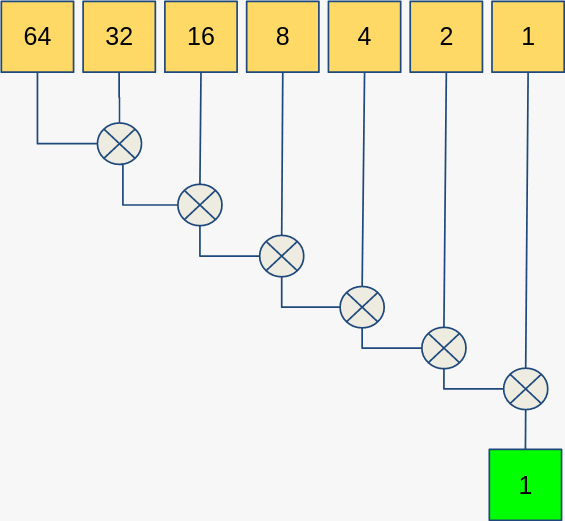
\includegraphics[width=0.5\textwidth]{ ./figures/fig3.png }
\caption*{\texttt{std::accumulate} }
\end{figure}	
\end{minipage}
\begin{minipage}{0.5\textwidth}
\begin{figure}[H]
\centering
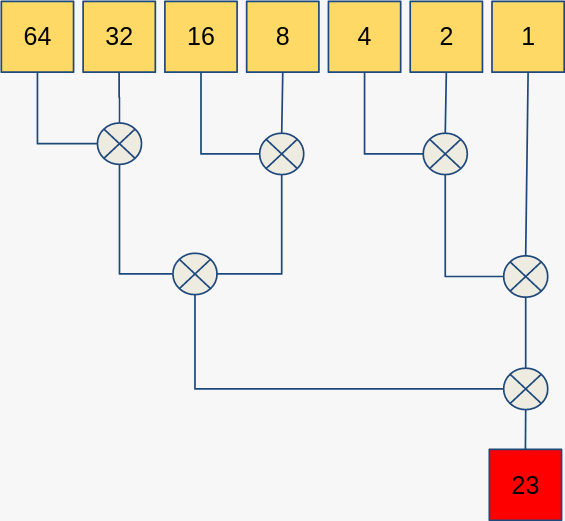
\includegraphics[width=0.5\textwidth]{ ./figures/fig4.png }
\caption*{\texttt{std::reduce} }
\end{figure}	
\end{minipage}
\bigbreak \noindent
With \texttt{std::reduce} we got the wrong answer because of the mathematical properties of subtraction. You can't abitrarily reorder the operands, or compute the operations out of order when doing subtraction. This is formalised in the properties of \textit{commutativity} and \textit{associativity}.
\bigbreak \noindent
With \texttt{std::reduce} the elements of the range may be grouped and rearranged in arbitrary order, which might break your code if the binary operation is not commutative and associative. 
\subsection{inner\_product}
\begin{minted}[linenos=false]{cpp}
template< typename InputIt1, typename InputIt2, typename T >
T inner_product( InputIt1 first1, InputIt1 last1,                         (1)
                 InputIt2 first2, T init );

template< typename InputIt1, typename InputIt2, typename T,
          typename BinaryOp1, typename BinaryOp2 >
T inner_product( InputIt1 first1, InputIt1 last1,                         (2) 
                 InputIt2 first2, T init, 
                 BinaryOp1 op1, BinaryOp2 op2 );
\end{minted}
\noindent Computes inner product (i.e sum of products) or performs ordered map/reduce operation on the range [first1, last1] and the range of \texttt{std::distance(first1,last1)} elements beginning at first2.
\begin{enumerate}
    \item Initializes the accumulator \texttt{acc} (of type T) with the initial value \texttt{init} and then modifies it with the expression \texttt{acc = std::move(acc) + (*i1) * (*i2)} for every iterator \texttt{i1} in the range [first1, last1] in order and its correspoinding iterator \texttt{i2} in the range beginning at \texttt{first2}. For built-in meaning of + and *, this computes inner product of the two ranges.
    \item Initializes the accumulator \texttt{acc} (of type T) with the initial value \texttt{init} and then modifies it with the expression \texttt{acc = op1(std::move(acc), op2(*i1,*i2))} for every iterator \texttt{i1} in the range [first1, last1] in order and its corresponding iterator \texttt{i2} in the range beginning at \texttt{first2}.
\end{enumerate}
The implementation might look something like this for the overload that accepts \textbf{no} binary function objects.
\begin{minted}[linenos=false]{cpp}
template<typename InputIt1, typename InputIt2, typename T>
constexpr 
T inner_product(InputIt1 first1, InputIt1 last1, InputIt2 first2, T init)
{
    while (first1 != last1)
    {
        init = std::move(init) + (*first1) * (*first2);
        ++first1;
        ++first2;
    }
    return init;
}
\end{minted}
For the version of \texttt{std::inner\_product} that takes two binary function objects. The implementation might look like this.
\begin{minted}[linenos=false]{cpp}
template<typename InputIt1, typename InputIt2, typename T
         typename BinaryOp1, typename BinaryOp2>
constexpr 
T inner_product(InputIt1 first1, InputIt1 last1, InputIt2 first2, T init, BinaryOp1 op1, BinaryOp2, op2)
{
    while (first1 != last1)
    {
        init = op1(std::move(init), op2(*first1,*first2));
        ++first1;
        ++first2;
    }
    return init;
}
\end{minted}
\newpage
Heres an example of \texttt{std::inner\_product in practice}
\begin{minted}[linenos=false]{cpp}
int main()
{
    std::vector<int> a{0,1,2,3,4};
    std::vector<int> b{5,4,3,2,1};

    int r1 = std::inner_product(a.begin(), a.end() b.begin(), 0);
    std::cout << "Inner product of a and b: " << r1 << "\n";

    int r2 = std::inner_product(a.begin(), a.end() b.begin(), 0, 
                                std::plus<>(), std::equal_to<>());
    std::cout << "Number of pairwise matches between a and b" << r2 << "\n";
}
\end{minted}
\noindent Output: 
\begin{mdframed}
Inner product of a and b: 21  \\
Number of pairwise matches between a and b: 2
\end{mdframed}
\noindent
Interestingly enough, you dont actually need 2 containers for \texttt{inner\_product}, if you pass the \texttt{first1} again as \texttt{first2}, you can apply a transformation on the same element twice. For example, say you wanted to calculate the sum of squares in a container, if your transfor
\section{transform\_reduce}
Just like how \texttt{std::reduce} is the parallelized version of \texttt{std::accumulute}, \texttt{transform\_reduce} is the parallelized version of \texttt{std::inner\_product}. This function has a wide range of parameter options.
\begin{minted}[linenos=false]{cpp}
// Default transform and reduce operations (multiple and add)
template <typename InputIt1, typename InputIt2, typename T> 
T transform_reduce (InputIt1 first1, InputIt1 last1, InputIt2 first2, T init);


// Takes two binary function objects.
template< typename InputIt1, typename InputIt2, typename T,
typename BinaryOp1, typename BinaryOp2 >
T transform_reduce( InputIt1 first1, InputIt1 last1,
                    InputIt2 first2, T init,
                    BinaryOp1 reduce, BinaryOp2 transform );

// Takes an Execution policy
template <typename ExecutionPolicy, typename ForwardIt1, typename ForwardIt2, typename T>
T transform_reduce(ExecutionPolicy&& policy, 
                   FowardIt1 first1, ForwardIt1 last1, ForwardIt2 first2, T init);

// Takes an Execution policy and two binary function objects.
template< typename ExecutionPolicy,
          typename ForwardIt1, typename ForwardIt2, typename T,
          typename BinaryOp1, typename BinaryOp2 >
T transform_reduce( ExecutionPolicy&& policy,
                    ForwardIt1 first1, ForwardIt1 last1,
                    ForwardIt2 first2, T init,
                    BinaryOp1 reduce, BinaryOp2 transform )

// Only requires one container
template< typename InputIt, typename T,
          typename BinaryOp, typename UnaryOp >
T transform_reduce( InputIt first, InputIt last, T init,
                    BinaryOp reduce, UnaryOp transform );

// One container, takes execution policy
template< typename ExecutionPolicy,
          typename ForwardIt, typename T,
          typename BinaryOp, typename UnaryOp >
T transform_reduce( ExecutionPolicy&& policy,
                    ForwardIt first, ForwardIt last, T init,
                    BinaryOp reduce, UnaryOp transform );

\end{minted}
Much like \texttt{std::inner\_product}, this algorithm will apply a transform operation on \texttt{first1, *first2}, and reduces the results (possibly permuted and aggregated in unspecified manner).
\nt{
    The result is non-deterministic if the reduce is not associative or not commutative (like with \texttt{std::reduce})
}
\section{partial\_sum}
\section{adjacent\_difference}
\end{document}
